\documentclass[11pt,a4paper]{ctexart}

\usepackage[margin=1in]{geometry}
\usepackage{booktabs}
\usepackage{longtable}
\usepackage{tabularx}
\usepackage{graphicx}
\usepackage{float}
\usepackage{hyperref}
\usepackage{xcolor}
\usepackage{enumitem}
\usepackage{amsmath}
\usepackage{siunitx}

\hypersetup{
  colorlinks=true,
  linkcolor=blue!55!black,
  citecolor=blue!55!black,
  urlcolor=blue!55!black
}

\setlist[itemize]{leftmargin=1.5em}
\setlist[enumerate]{leftmargin=1.8em}
\emergencystretch=3em
\Urlmuskip=0mu plus 2mu
\newcommand{\todo}[1]{\textcolor{red}{#1}}
\newcommand{\githuburl}{\todo{待填写：GitHub 仓库链接}}
\newcommand{\weightsurl}{\todo{待填写：模型权重网盘链接}}

\title{\textbf{题目二：基于 LeRobot 的 ACT 策略跨环境泛化挑战}}
\author{
  小组成员：\todo{姓名 / 学号待填写}\\
  分工情况：\todo{待填写：数据准备、训练评估、报告撰写等具体分工}\\
  项目仓库：\githuburl\\
  模型权重：\weightsurl
}
\date{2026 年 5 月}

\begin{document}
\maketitle

\begin{abstract}
本报告完成作业题目二中基于 LeRobot 的 ACT（Action Chunking Transformer）跨环境泛化实验。实验在 CALVIN 数据集上构造两条可比的行为克隆训练线：第一条仅使用环境 A 数据训练视觉-动作策略，记为 ACT-A；第二条混合环境 A、B、C 数据训练同构策略，记为 ACT-ABC。两者采用完全相同的 ACT 网络结构与训练超参数，并在未参与训练的环境 D 上进行 zero-shot 动作误差评估。实验结果显示，虽然 ACT-A 在单一环境训练集上的最终训练 loss 更低，但在环境 D 的最终 checkpoint 上，ACT-ABC 的 offline Action L1 为 0.2757，低于 ACT-A 的 0.2990，相对下降约 7.79\%。这表明多环境联合训练能缓解部分视觉分布偏移，提高跨环境泛化表现。同时，checkpoint 曲线显示最佳 D-D 动作误差并不总出现在最终训练步，提示行为克隆策略在源环境上继续收敛时可能出现对源视觉分布的过拟合。
\end{abstract}

\section{任务背景}
具身智能策略学习需要从视觉、机器人状态和语言任务等多模态观测中预测连续动作。单环境行为克隆模型往往能在训练分布内快速收敛，但部署到未见过的视觉场景时会受到背景、光照、物体位置与相机观测差异的影响。作业题目二要求使用 LeRobot 框架中集成的轻量级 ACT 算法，在 CALVIN 数据集上比较单环境训练和多环境联合训练的跨环境泛化能力。

本实验只针对题目二，核心问题包括：
\begin{enumerate}
  \item 仅使用环境 A 数据训练的 ACT 策略是否能泛化到完全未见过的环境 D；
  \item 使用环境 A+B+C 数据联合训练是否能提高 zero-shot 到环境 D 的动作预测质量；
  \item ACT 的动作分块机制在视觉分布偏移下体现出哪些鲁棒性和局限。
\end{enumerate}

\section{数据集描述}
实验使用 Hugging Face 上 LeRobot v2.1 格式的 CALVIN 数据。原始 \texttt{fywang/calvin-task-ABC-D-lerobot} 数据集中包含官方 training split 的 A/B/C 场景以及末尾的 D validation 场景。为了保证环境 D 是 zero-shot 目标域，本实验根据官方 \texttt{task\_ABC\_D} metadata 重新切分，只保留官方 training split 中的 A/B/C episode，并进一步抽取只属于环境 A 的 episode。

\begin{table}[H]
\centering
\caption{训练与测试数据划分。}
\begin{tabular}{llrrl}
\toprule
数据集 & 用途 & Episodes & Frames & 场景组成 \\
\midrule
\texttt{local/calvin-task-A-train-lerobot} & ACT-A 训练 & 6,089 & 366,693 & A \\
\texttt{local/calvin-task-ABC-train-lerobot} & ACT-ABC 训练 & 17,870 & 1,071,743 & A=6,089, B=6,115, C=5,666 \\
\texttt{fywang/calvin-task-D-D-lerobot} & zero-shot 测试 & 6,135 & 369,493 & D \\
\bottomrule
\end{tabular}
\end{table}

每个样本包含两个视觉观测、机器人状态、环境状态、语言任务和连续动作。主要输入输出如下：
\begin{itemize}
  \item 顶部相机图像：\texttt{observation.images.top}，尺寸为 $3 \times 200 \times 200$；
  \item 手腕相机图像：\texttt{observation.images.wrist}，尺寸为 $3 \times 84 \times 84$；
  \item 机器人状态：\texttt{observation.state}，维度为 15；
  \item 动作：\texttt{action}，维度为 7；
  \item 帧率：10 FPS。
\end{itemize}

\section{方法}
\subsection{LeRobot 行为克隆流程}
LeRobot 提供统一的数据读取、策略配置、训练循环和 checkpoint 管理接口。本实验使用 LeRobot v0.3.3 读取 v2.1 数据格式，在固定离线数据集上训练 ACT 策略。训练时使用 ImageNet 图像归一化统计量，关闭在线环境交互评估，按固定步数保存 checkpoint。

\subsection{ACT 策略结构}
ACT 使用视觉编码器和 Transformer 结构从当前观测预测未来一段动作序列。相比逐步预测单个动作，ACT 一次预测动作块（action chunk），使模型能学习短时动作轨迹结构，减少逐帧决策带来的抖动。

本实验采用的 ACT 配置如下：
\begin{table}[H]
\centering
\caption{ACT 网络结构与训练超参数。ACT-A 与 ACT-ABC 完全一致。}
\begin{tabularx}{\linewidth}{lX}
\toprule
项目 & 设置 \\
\midrule
Policy & ACT, LeRobot v0.3.3 \\
视觉骨干 & ResNet-18 \\
Transformer hidden dimension & 512 \\
Feedforward dimension & 3,200 \\
Attention heads & 8 \\
Encoder / Decoder layers & 4 / 1 \\
VAE encoder layers / latent dim & 4 / 32 \\
Action dimension & 7 \\
Observation state dimension & 15 \\
Chunk size / action steps & 10 / 10 \\
Observation steps & 1 \\
Normalization & Action/State/Visual: mean-std normalization \\
Optimizer & AdamW, $\beta=(0.9,0.999)$, weight decay $10^{-4}$ \\
Learning rate & $1\times10^{-5}$ \\
Batch size & 64 \\
Training steps & 200,000 \\
Gradient clipping & 10.0 \\
Checkpoint frequency & 5,000 steps \\
Training loss & ACT reconstruction/action loss with VAE KL regularization, KL weight 10 \\
Evaluation metric & Offline unnormalized Action L1 on environment D \\
\bottomrule
\end{tabularx}
\end{table}

\section{实验设置}
\subsection{硬件与软件环境}
实验在单张 NVIDIA GeForce RTX 3060 12GB GPU 上完成。软件环境为 Python 3.10.20、PyTorch 2.5.1+cu121、CUDA 12.1、LeRobot v0.3.3。LeRobot main/v0.5 系列默认面向 Python 3.12 与 v3.0 数据格式，因此本实验选择兼容 CALVIN-LeRobot v2.1 数据的 v0.3.3 版本。

\subsection{训练设置}
ACT-A 使用环境 A 的 6,089 个 episode 训练；ACT-ABC 使用环境 A/B/C 的 17,870 个 episode 训练。两者 batch size、学习率、优化器、模型结构和训练步数保持一致。由于 ACT-A 数据量更小，同样 200,000 steps 对应约 34.90 epochs；ACT-ABC 对应约 11.94 epochs。

\subsection{Zero-shot 环境 D 测试}
PDF 要求在环境 D 上评估成功率（Success Rate）或动作误差。本实验采用动作误差作为 zero-shot 泛化指标：对 D-D 数据集的观测输入，使用 checkpoint 预测动作块，并与数据集中专家动作计算 unnormalized Action L1。每个 checkpoint 评估 200 个 batch，每个 batch 64 个样本，共 12,800 个样本。该指标不等同于闭环 rollout success rate，但能直接衡量模型在未见视觉域中复现专家动作的能力。

\section{实验结果}
\subsection{图表记录方式}
课程提交要求使用 WandB 或 SwanLab 导出训练与验证曲线。为严格满足该要求，本实验将原始 LeRobot 训练日志和环境 D 评估 JSON 解析为标量 CSV 后，使用 \texttt{scripts/log\_swanlab\_from\_csv.py} 将 ACT-A 与 ACT-ABC 分别 replay 为两个 SwanLab local experiments，并通过 \texttt{swanlab watch} 的 dashboard 导出曲线图。报告中的训练 loss、D-D Action L1 和总览面板均为 SwanLab dashboard 导出图；曲线源数据保存在 \path{report/tables/act_training_loss.csv} 和 \path{report/tables/act_dd_l1_by_checkpoint.csv}。

\subsection{训练收敛曲线}
图 \ref{fig:swanlab_train_dd} 左图给出 SwanLab dashboard 导出的训练 loss 平滑曲线。由于训练最初数千 step 存在很大的 warmup 尖峰，主图展示 5K step 之后的 median-400 平滑 loss，便于比较主体收敛趋势。ACT-A 的训练 loss 下降更快、最终更低，最终解析日志 loss 约为 0.164；ACT-ABC 最终训练 loss 约为 0.228。这一现象符合预期：ACT-A 只拟合单一视觉环境，数据分布更窄；ACT-ABC 同时拟合 A/B/C 三种环境，任务难度和视觉多样性更高。

\begin{figure}[H]
\centering
\begin{minipage}{0.48\linewidth}
\centering
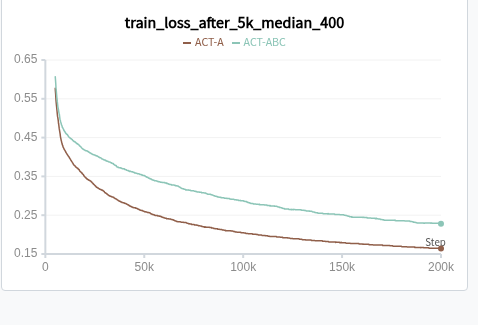
\includegraphics[width=\linewidth]{figures/swanlab_train_loss_after_5k.png}
\end{minipage}
\hfill
\begin{minipage}{0.48\linewidth}
\centering
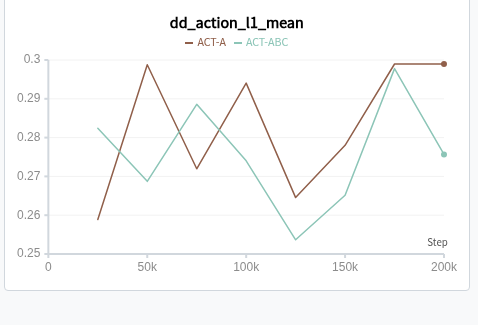
\includegraphics[width=\linewidth]{figures/swanlab_dd_l1_mean.png}
\end{minipage}
\caption{SwanLab dashboard 导出的训练 loss 与环境 D zero-shot 验证曲线。左图为 5K step 之后的训练 loss median-400 平滑曲线；右图为不同 checkpoint 在 D-D 上的 offline Action L1 mean，数值越低表示预测动作越接近专家动作。}
\label{fig:swanlab_train_dd}
\end{figure}

图 \ref{fig:swanlab_dashboard} 给出 SwanLab dashboard 的整体截图，包含 raw loss、平滑 loss、梯度范数、学习率以及 D-D Action L1 mean/last 等曲线。可以看到，两条训练曲线均在初期快速下降，之后进入缓慢收敛阶段。

\begin{figure}[H]
\centering
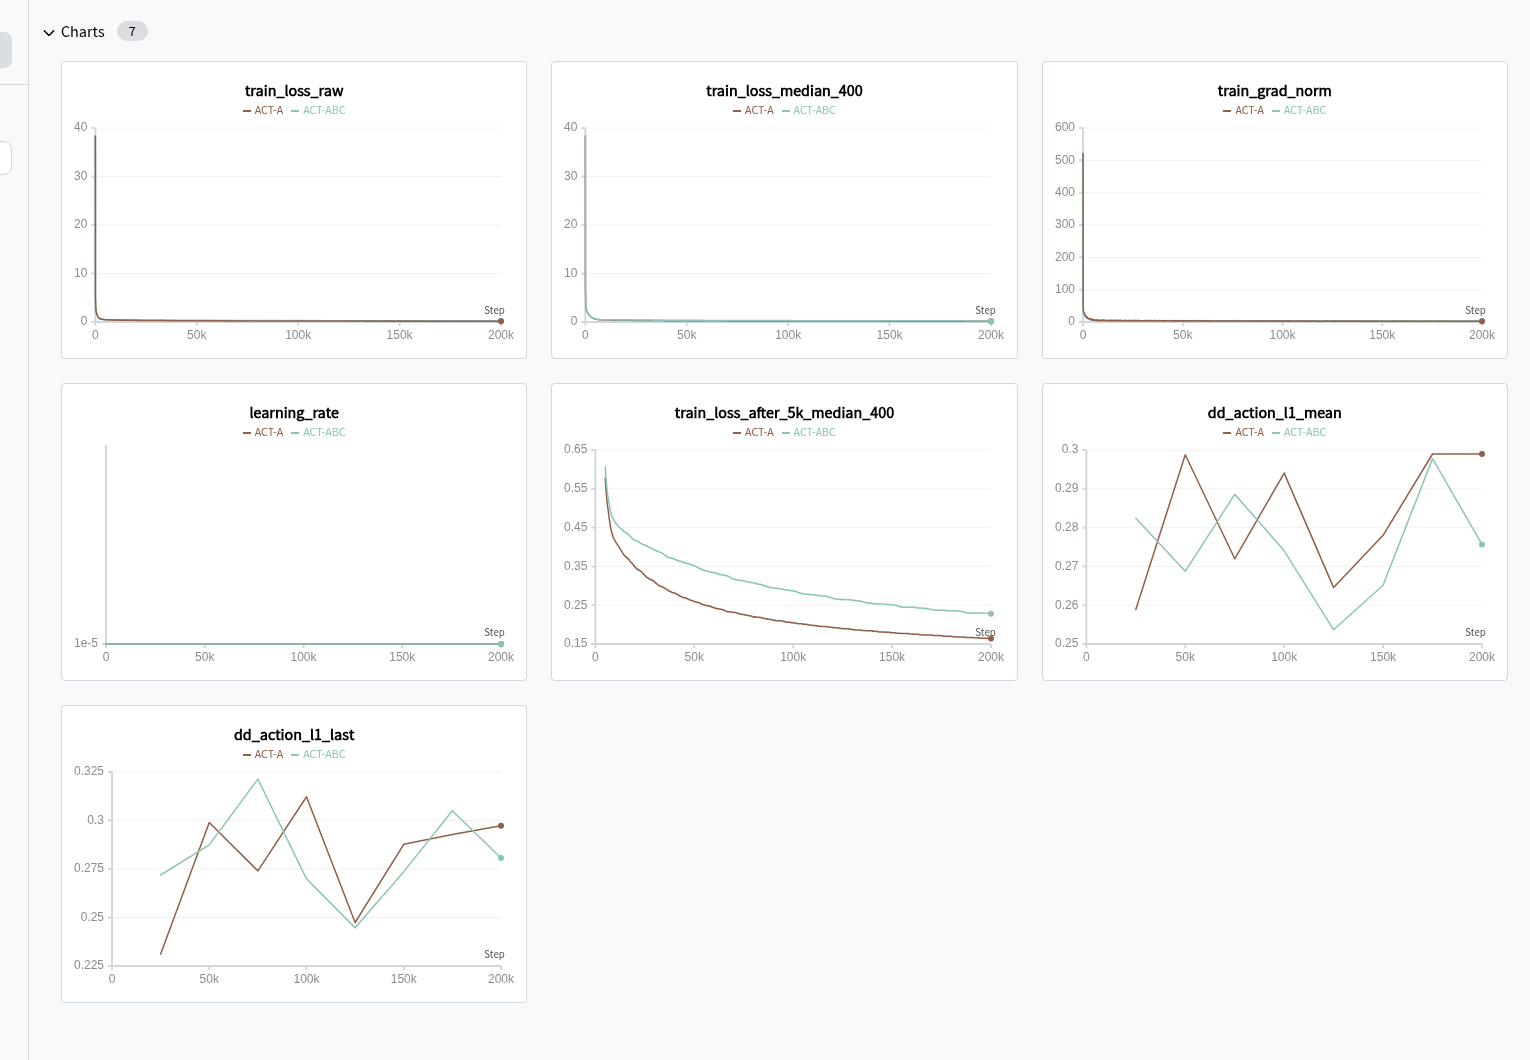
\includegraphics[width=\linewidth]{figures/swanlab_dashboard_curves.png}
\caption{SwanLab dashboard 导出的完整曲线面板截图。}
\label{fig:swanlab_dashboard}
\end{figure}

\subsection{环境 D 动作误差}
图 \ref{fig:swanlab_train_dd} 右图和表 \ref{tab:dd_l1} 汇总了两个模型在环境 D 上的 checkpoint 曲线。ACT-A 的最佳 D-D L1 出现在 25K step，为 0.2589；ACT-ABC 的最佳 D-D L1 出现在 125K step，为 0.2537。最终 200K checkpoint 上，ACT-ABC 的 D-D L1 为 0.2757，明显低于 ACT-A 的 0.2990。

\begin{longtable}{lrrrr}
\caption{D-D offline Action L1 详细结果。每个 checkpoint 评估 12,800 个样本。}
\label{tab:dd_l1}\\
\toprule
模型 & Step & D-D L1 Mean & D-D L1 Last & Samples \\
\midrule
\endfirsthead
\toprule
模型 & Step & D-D L1 Mean & D-D L1 Last & Samples \\
\midrule
\endhead
ACT-A & 25,000 & 0.2589 & 0.2311 & 12,800 \\
ACT-A & 50,000 & 0.2988 & 0.2990 & 12,800 \\
ACT-A & 75,000 & 0.2720 & 0.2740 & 12,800 \\
ACT-A & 100,000 & 0.2940 & 0.3122 & 12,800 \\
ACT-A & 125,000 & 0.2645 & 0.2474 & 12,800 \\
ACT-A & 150,000 & 0.2780 & 0.2877 & 12,800 \\
ACT-A & 175,000 & 0.2990 & 0.2928 & 12,800 \\
ACT-A & 200,000 & 0.2990 & 0.2973 & 12,800 \\
ACT-ABC & 25,000 & 0.2824 & 0.2719 & 12,800 \\
ACT-ABC & 50,000 & 0.2687 & 0.2874 & 12,800 \\
ACT-ABC & 75,000 & 0.2886 & 0.3213 & 12,800 \\
ACT-ABC & 100,000 & 0.2740 & 0.2699 & 12,800 \\
ACT-ABC & 125,000 & 0.2537 & 0.2447 & 12,800 \\
ACT-ABC & 150,000 & 0.2651 & 0.2736 & 12,800 \\
ACT-ABC & 175,000 & 0.2978 & 0.3051 & 12,800 \\
ACT-ABC & 200,000 & 0.2757 & 0.2807 & 12,800 \\
\bottomrule
\end{longtable}

\begin{table}[H]
\centering
\caption{最终 200K checkpoint 对比。}
\begin{tabular}{lrrr}
\toprule
模型 & 训练集 & Final Train Loss & D-D L1 Mean \\
\midrule
ACT-A & A & 0.164 & 0.2990 \\
ACT-ABC & A+B+C & 0.228 & 0.2757 \\
\bottomrule
\end{tabular}
\end{table}

在最终 checkpoint 上，ACT-ABC 相比 ACT-A 的 D-D L1 绝对下降 0.0233，相对 ACT-A 下降约 7.79\%。因此，从最终模型部署的角度看，多环境联合训练提高了环境 D 上的 zero-shot 动作预测质量。

\section{现象分析}
\subsection{单环境收敛更快但泛化更弱}
ACT-A 的训练 loss 更低，说明模型更容易拟合单一环境 A 的视觉和动作分布。然而该优势没有转化为环境 D 上的最终动作误差优势。环境 D 的背景纹理、相机观测、物体外观上下文与环境 A 存在分布偏移，单环境训练容易把视觉编码器和动作预测头绑定到源环境特征上，从而削弱跨环境表现。

\subsection{多环境训练提高最终 zero-shot 表现}
ACT-ABC 同时观察 A/B/C 三个环境，训练分布更宽，模型更难依赖单一背景或光照线索。虽然这使训练 loss 更高，但能迫使视觉编码器学习更稳定的任务相关特征，例如末端执行器、目标物体和相对位姿。最终 D-D L1 低于 ACT-A，说明多环境训练对未见环境 D 有正向泛化作用。

\subsection{最佳 checkpoint 早于最终 checkpoint}
两个模型的 D-D 曲线都不是单调下降。ACT-A 在 25K 和 125K 处较好，后期 D-D L1 升高；ACT-ABC 在 125K 处达到最佳，然后 175K 变差，200K 又有所恢复。这说明源域训练 loss 继续下降并不必然带来目标域动作误差下降。对行为克隆而言，模型可能在后期更精细地拟合源环境视觉细节，而这些细节在目标环境 D 中不稳定。因此，若以跨环境部署为目标，最好保留多个 checkpoint 并根据 held-out 目标域 proxy 或真实 rollout 指标选择模型。

\section{Action Chunking 在视觉偏移下的鲁棒性}
ACT 的 Action Chunking 将单步动作预测扩展为长度为 10 的动作块预测。该机制在跨环境视觉偏移下有两个潜在优势：
\begin{itemize}
  \item \textbf{短时轨迹先验。} 机器人操作任务通常具有连续、平滑的动作结构。一次预测未来 10 步动作能让模型学习动作序列中的短时一致性，减少逐帧视觉噪声导致的动作抖动。
  \item \textbf{降低局部观测敏感性。} 当单帧图像出现轻微视觉偏移时，动作块中的后续动作仍受到整体轨迹模式约束，因此对局部噪声有一定缓冲。
\end{itemize}

但 Action Chunking 也有局限：
\begin{itemize}
  \item 如果视觉编码器在新环境中错误定位目标或误判场景状态，整个动作块都可能朝错误方向偏移，错误会持续多个时间步；
  \item 离线 Action L1 只能衡量与专家动作的接近程度，不能评估闭环执行中的恢复能力；
  \item chunk size 固定为 10，若任务需要更长时程的纠错和探索，仅靠短动作块不足以解决严重视觉分布偏移。
\end{itemize}

\section{复现说明与开源链接}
本项目仓库根目录提供 README、环境配置、数据准备说明、训练命令和测试命令。权重文件体积较大，不放入 GitHub 仓库，需通过云盘链接下载。

\begin{itemize}
  \item 项目 GitHub 仓库：\githuburl
  \item 模型权重下载：\weightsurl
  \item SwanLab 训练曲线：\path{report/figures/swanlab_train_loss_after_5k.png}
  \item SwanLab 验证曲线：\path{report/figures/swanlab_dd_l1_mean.png}
  \item SwanLab 总览面板：\path{report/figures/swanlab_dashboard_curves.png}
  \item 指标 CSV：\texttt{report/tables/act\_dd\_l1\_by\_checkpoint.csv}
\end{itemize}

\section{结论}
本实验完成了题目二要求的两条 ACT 策略训练线和环境 D zero-shot 测试。结果表明，单环境 ACT-A 在源训练集上收敛更快、训练 loss 更低，但最终 checkpoint 在未见环境 D 上的动作误差较高；多环境 ACT-ABC 尽管训练 loss 更高，却在最终 D-D 动作误差上更优。该结果支持多环境联合训练能够提高视觉-动作策略跨环境泛化能力的结论。同时，Action Chunking 提供了短时动作平滑和轨迹先验，但在严重视觉分布偏移下仍依赖视觉编码器是否能提取稳定的任务相关特征。未来若计算资源允许，可进一步接入 CALVIN 仿真环境，补充真实闭环 rollout success rate。

\begin{thebibliography}{9}
\bibitem{calvin}
Mees, O., Hermann, L., Rosete-Beas, E., and Burgard, W. CALVIN: A Benchmark for Language-Conditioned Policy Learning for Long-Horizon Robot Manipulation Tasks.
\bibitem{act}
Zhao, T. Z., Kumar, V., Levine, S., and Finn, C. Learning Fine-Grained Bimanual Manipulation with Low-Cost Hardware.
\bibitem{lerobot}
Hugging Face. LeRobot: State-of-the-art Machine Learning for Real-World Robotics.
\end{thebibliography}

\end{document}
